
\section{Pinhole Camera Model}

The pinhole camera model describes the mathematical relationship between the points of the image plane and the 3D points captured by an 
ideal pinhole camera. In the context of this work, this model is useful to explain how the depth is calculated by Kinect and 
how to re-project points in the photo-consistency method.

\begin{figure}[H]
\begin{center}
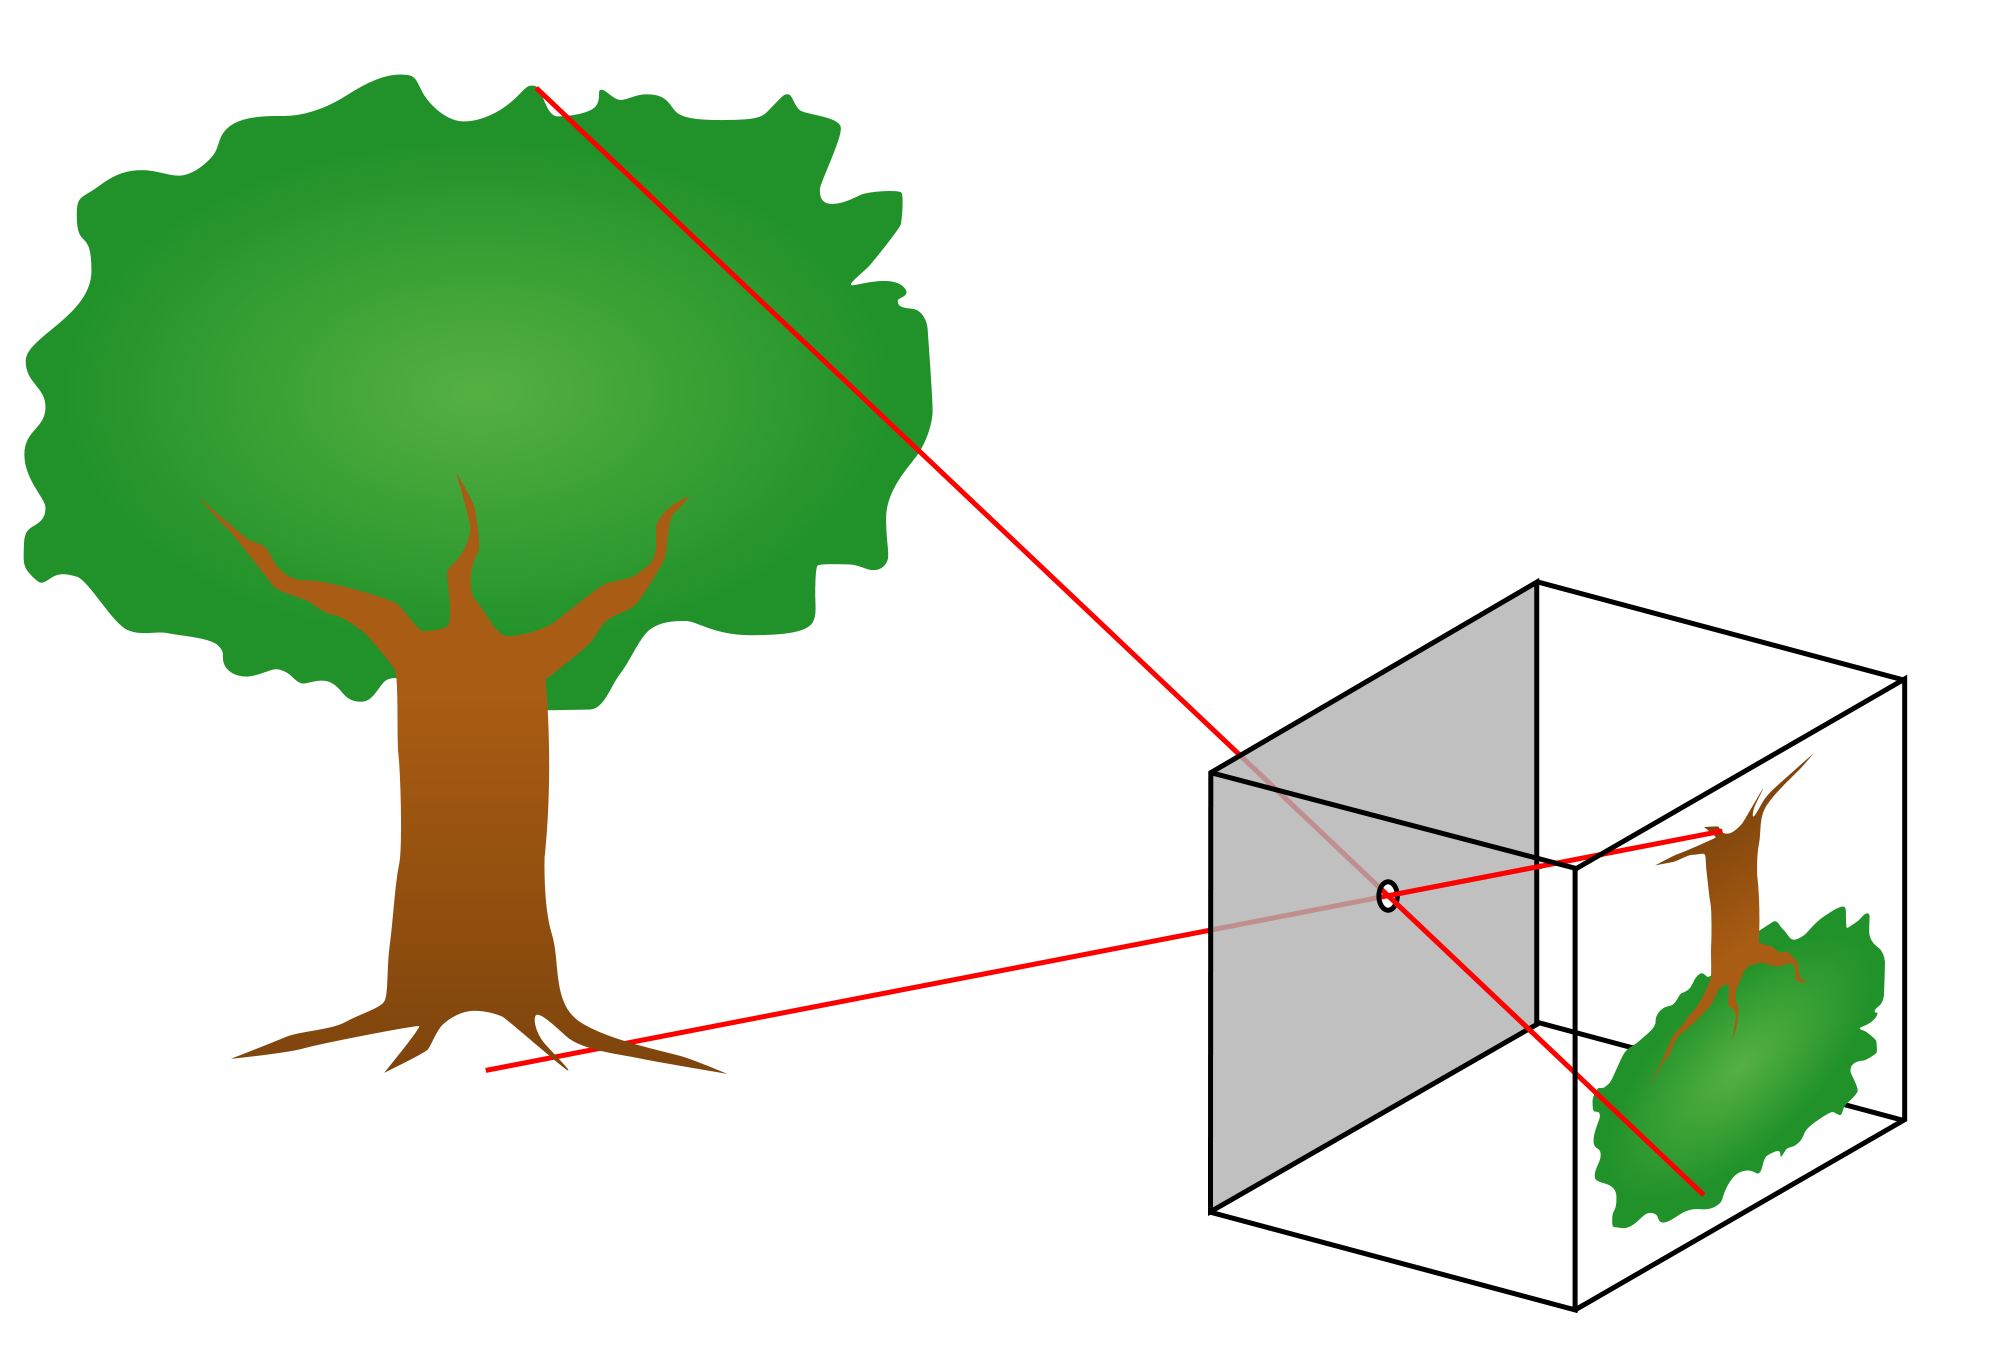
\includegraphics[scale=0.15]{images/pinhole-camera}
\caption{Pinhole camera.}
\label{fig:pinhole}
\end{center}
\end{figure}

In the pinhole camera all rays pass from the scene to a photosensitive material through a pinhole, in order to form the image.

\begin{figure}[H]
\begin{center}
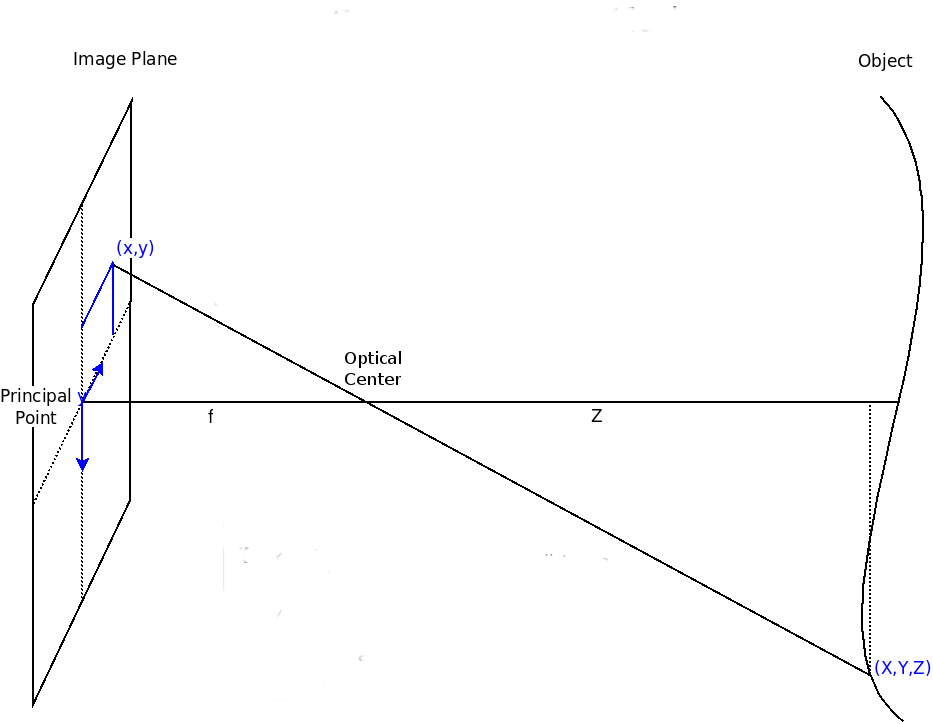
\includegraphics[scale=1]{images/pinhole-coordinates}
\caption{Pinhole camera coordinates system.}
\label{fig:pinhole-c}
\end{center}
\end{figure}

In \ref{fig:pinhole-c} the point $P$ denotes the principal point, $O$ is the optical center and 
$f=dist(P,O)$ is the focal length.

The transformation between world coordinates point $(X,Y,Z)$ and image coordinates $(x,y)$ is described as 
follows:

\begin{equation}
\label{eq:disparity2}
 x = \frac{fX}{Z}\ ,
\end{equation}

\begin{equation}
\label{eq:disparity2}
 y = \frac{fY}{Z}\ .
\end{equation}

These equations are  obtained using triangles similarity.

\section{Kinect Sensor}

Kinect sensor was launched at the end of 2010 by Microsoft. A structured light camera 
used as peripheral for the Xbox 360. With sales of more than 24 million devices at February 2013.
The sensor gained great attention from computer vision and robotics communities, because it offers 
accurate depth information at low cost in comparison to existing alternatives.

\section{Sensor Depth Calculation}

The Kinect sensor consists of an infrared laser emitter, an 
infrared camera and an RGB camera. Both cameras can work up to 30Hz. 
The laser source emits a single 
beam which is split into multiple beams by a diffraction 
grating to create a constant 
pattern of speckles projected onto the scene. This pattern is 
captured by the infrared camera and is correlated against a 
reference pattern. The reference pattern is obtained by capturing 
a plane at a known distance from the sensor, and is stored in the 
memory of the sensor. When a speckle is projected on an object 
whose distance to the sensor is smaller or larger than that of the 
reference plane the position of the speckle in the infrared image 
will be shifted in the direction of the baseline between the laser 
projector and the perspective center of the infrared camera. 
These shifts are measured for all speckles by a simple image 
correlation procedure, which yields a disparity image \cite{khoshelham2011accuracy}. For each 
pixel the distance to the sensor can then be retrieved from the 
corresponding disparity.



\begin{figure}[h!]
\begin{center}
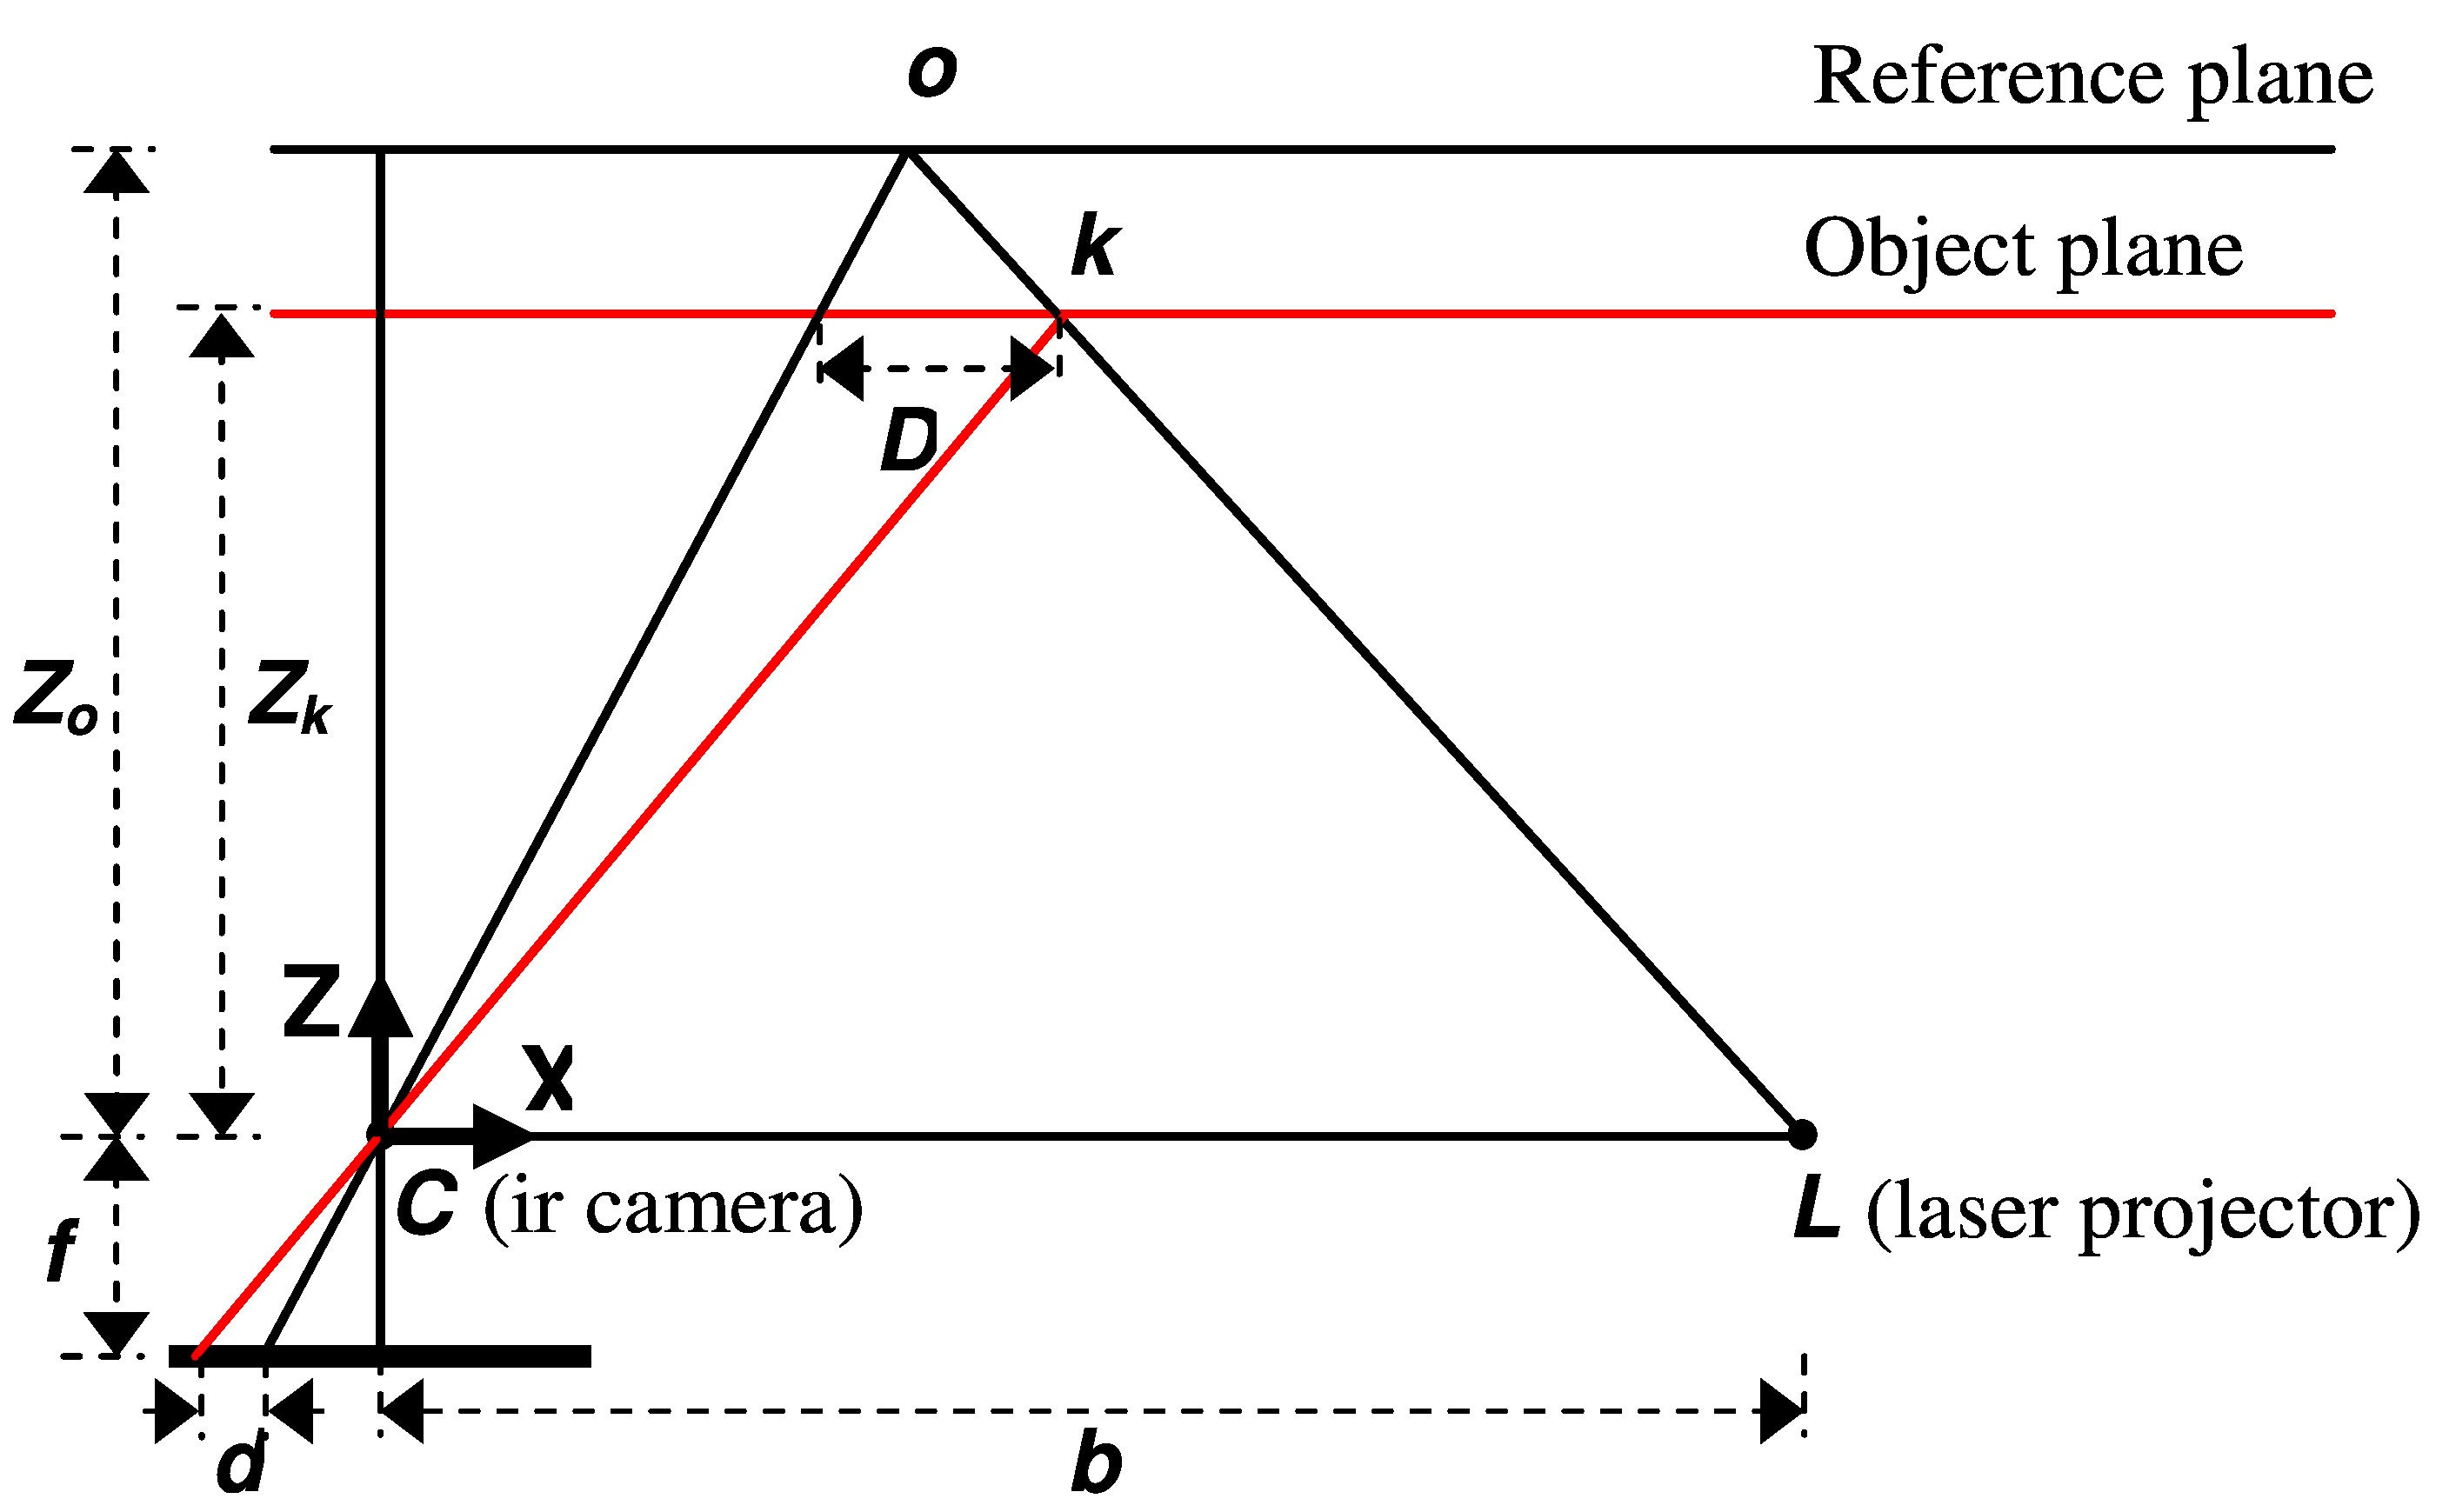
\includegraphics[scale=1.65]{images/kinect_triangulation}
\caption{Schematic representation of depth-disparity relation. Image taken from \cite{khoshelham2011accuracy}.}
\label{fig:disparity}
\end{center}
\end{figure}

\begin{equation}
\label{eq:disparity1}
 \frac{D}{b} = \frac{Z_0 - Z_k}{Z_0}\ ,
\end{equation}


\begin{equation}
\label{eq:disparity2}
 \frac{d}{f} = \frac{D}{Z_k}\ . 
\end{equation}

Then $Z_k$ can be obtained from \ref{eq:disparity1} and \ref{eq:disparity2}. Where variables $Z_0$,$b$ and $f$ are known.

\section{Sensor Captured Data}
\label{sec:sensor_data}

The sensor obtains two images: An RGB color image and a depth map. 

The RGB color image has three channels: Red, Green and Blue. And each image color is generated 
combining this three colors. With a resolution of 640x480 pixels and 1 byte per channel. The sensor can 
capture color images at higher resolutions, but in our case we need just one color per depth map pixel.

The depth map is like a gray scale image, where the value of each pixel is the object distance to the sensor in the viewing axis. 
A depth map is an image with a resolution of 640x480 and one channel of 2 bytes. We use meters as distance unit.

\begin{figure}[H]
\begin{center}
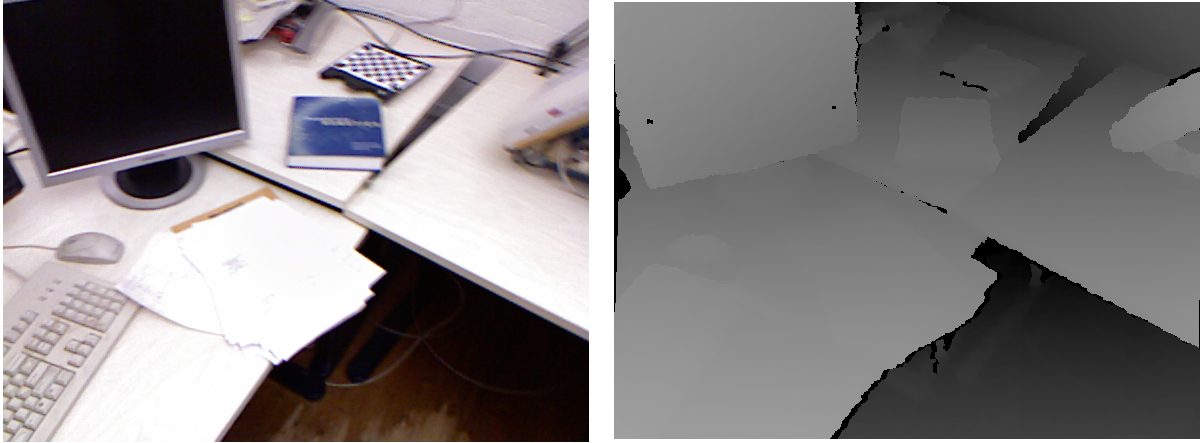
\includegraphics[scale=0.3]{images/color_depth.png}
\caption{Left: RGB image. Right: depth map converted to a grayscale image (0-255 values) for visualization purposes.}
\label{fig:colordepth}
\end{center}
\end{figure}


\begin{figure}[H]
\begin{center}
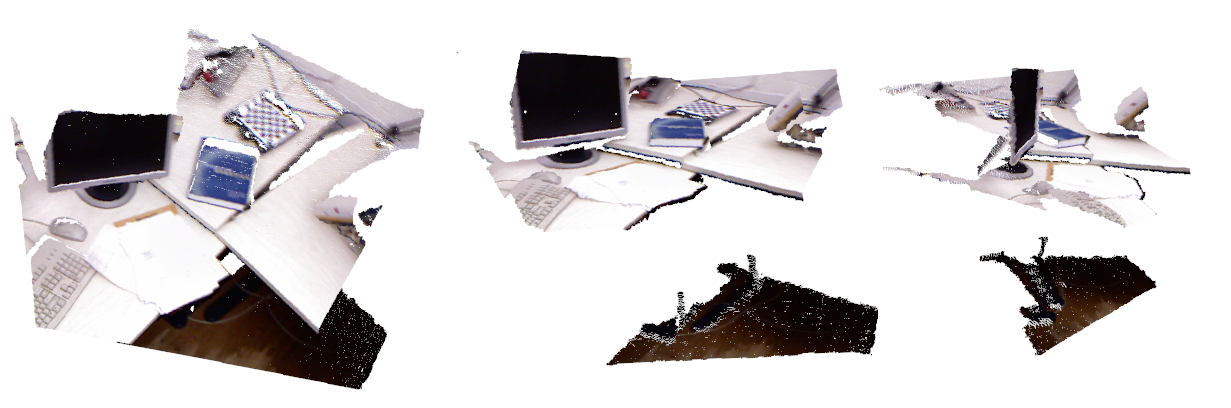
\includegraphics[scale=0.25]{images/3d_point_cloud.png}
\caption{Different perspectives of 3D color point cloud obtained by combining the RGB image colors and the depth map 3D points.}
\label{fig:colorpcloud}
\end{center}
\end{figure}


The depth map implicitly contains the object's world coordinates, the relation between depth map 
and world coordinates is described as follows:

\begin{equation}
\label{eq:depthmapx}
 X=\frac{(x-x')Z}{f}\ ,
\end{equation}

\begin{equation}
\label{eq:depthmapy}
 Y=\frac{(y-y')Z}{f}\ ,
\end{equation}


\noindent where $(x',y')$ is the image principal point (projection of optical center on the image plane), $f$ is the camera 
focal length, $(x,y)$ are the 2D coordinates in the depth map plane (640 pixels width, 480 pixels height) and $Z$ is the distance in the viewing axis from the camera to the object that is in position $(x,y)$ of the depth map.

\begin{figure}[H]
\begin{center}
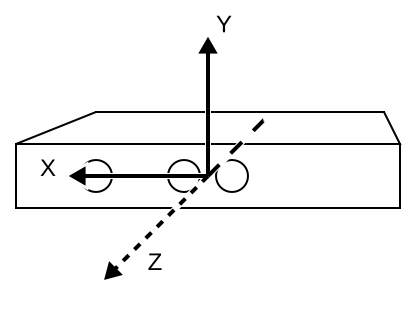
\includegraphics[scale=0.55]{images/coordinates}
\caption{Kinect coordinates system.}
\label{fig:coordinates}
\end{center}
\end{figure}

In this work we will use the RGB image, the depth map and the point cloud obtained combining both. The concept depth map pixel will 
refer to a discrete $(x,y)$  location on the depth map plane with a z-axis distance in meters and a 3D point will be a $(X,Y,Z)$ coordinate, 
obtained converting $(x,y)$ values to $(X,Y)$ using previous equations, along with the z-axis distance of the depth map as $Z$ component.
 
RGB camera has a slightly larger angle of view than the depth camera, for this reason a calibration must be done 
in order to have RGB images and depth maps using the same coordinates. The dataset already has RGB images and depth maps 
calibrated. More information about 
this process can be found in \cite{sturm12iros}.
